%\documentclass[11pt]{report}
%\linespread{1.3} %1.3 for one and a half spacing, 1.6 for double
%\usepackage{amsmath, amsthm, amssymb,float, graphicx, caption, subcaption, cite, braket, url, color}
%%\usepackage[nohug,heads=vee]{diagrams}
%%\diagramstyle[labelstyle=\scriptstyle]
%%\graphicspath{{./Figures/}}
%\usepackage[margin=2.5cm]{geometry}
%%\title{Title}
%%\author{Chrysoula Vlachou}
%%\date{}
%\newtheorem{lemma}{Lemma}
%\newtheorem{theorem}{Theorem}
%\newtheorem{proposition}{Proposition}
%%\theoremstyle{definition}
%\newtheorem{definition}{Definition}
%\newtheorem{protocol}{Protocol}
%%\newtheorem*{post}{Postulate}
%%\newtheorem*{rmrk}{Remark}
%%
%\newcommand{\N}{\mathbb N}
%\newcommand{\R}{\mathbb R}
%\newcommand{\C}{\mathbb C}
%\newcommand{\Hilb}{\mathcal H}
%\newcommand{\HRule}{\rule{\linewidth}{0.5mm}}
%\newcommand{\mmobh}{\textlatin{M\"ob}(\mathbb{H})}
%\newcommand{\areah}{\textlatin{area}_{\mathbb{H}}}
%\newcommand{\dth}{d_{\mathbb{H}}}
%\newcommand{\tdth}{$d_{\mathbb{H}}$ }
%\def\h{\mathbb H}
%\DeclareMathOperator{\tr}{Tr}
%\def\I{\hat I}
%\def\ds{\displaystyle}
%\def\ppmod{\!\!\!\!\!\pmod}
%\newcommand{\walkop}{U_{\text{walk}}}
%
%\def\poly{poly}
%\def\span{span}
%\def\O{\textbf{\textit{O}}}
%\newcommand{\innerproduct}[2]{\langle #1 | #2 \rangle}
%\def\mobh{\textlatin{M\"ob}({\mathbb H})}
%\def\span{span}
%
%
%\begin{document}
\chapter{Quantum key distribution based on quantum walks}

In this chapter, we present three new QKD protocols based on QWs. In particular, in Section~\ref{sec:qkdscheme}, we propose a secure two-way QKD scheme based on QWs, which is a modification of the public-key cryptosystem that was presented in the previous chapter. We equip this protocol with two different verification procedures against full man-in-the-middle attacks. In Section~\ref{sec:oneway}, we introduce a one-way QKD protocol of the BB84 type, which we prove to be secure against general attacks, by reducing it to an equivalent entanglement-based protocol. We also provide numerical results for the optimal choice of the QW parameters that maximise its noise tolerance. In Section~\ref{sec:semi-qkdscheme} we provide a semi-quantum key distribution (SQKD) protocol and show its robustness against eavesdropping. We comment on the efficiency and the quantum memory requirements for all these protocols and in Section~\ref{sec:prac_att}, we discuss some possible practical attacks. In the last section, we summarise our results and suggest relevant directions of future work.

\vfill

\begin{center}
 *The work presented in this chapter corresponds to the work published in~\cite{vla:kra:mat:pau:sou:17}.
\end{center}

\newpage



\section{Two-way quantum key distribution protocol}
\label{sec:qkdscheme}
In this section, we revisit the QW public-key cryptosystem presented in Chapter 2, in order to construct a secure two-way QKD protocol. We suitably modify it, so that the quantum state generated by means of a QW encodes a key instead of a message; such a key could be used later as input to a one-time-pad encryption system. However, this modification is non-trivial and requires care, since we can no longer rely on the existence of a trusted mechanism for public-key delivery (a public-key infrastructure, for instance), as it is typically assumed in quantum public-key cryptography~\cite{nik:08,sey:nik:alb:12}. 
Our motivation for modifying the original public-key protocol is the fact that QKD schemes are quite flexible, as the key can be used by both $A$ and $B$ to send or authenticate messages. Also, more post-processing techniques (e. g. privacy amplification) can be applied, since we have as input a random string and not a plaintext message. In the latter case, we should be careful during the post-processing not to degrade the message (we are left with less techniques). Furthermore, in the case of information leakage, we can safely abort the protocol, while during message transmission it would be late for that.
Our two-way protocol is depicted in Figure~\ref{fig:protQKD} and presented below. We assume that the key can be chosen among $P$ possible keys. We also assume that the QW can be chosen from a prefixed discrete set known by both parties. 



\begin{center}
\begin{figure}[!h]
  \centering
  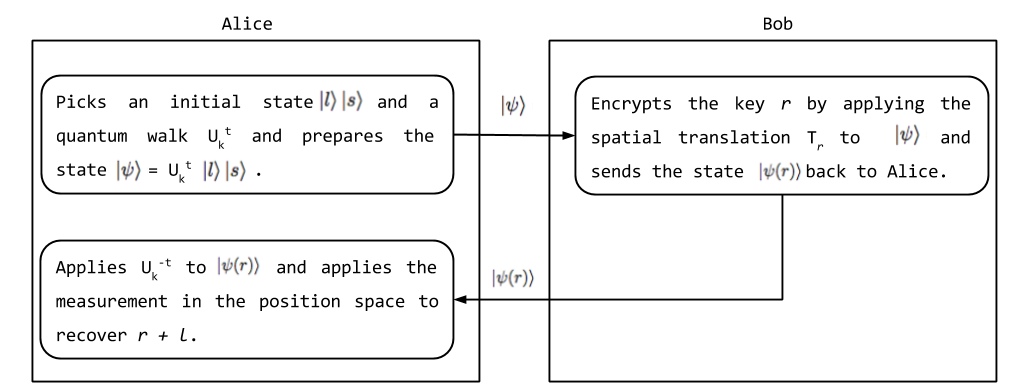
\includegraphics[width=\textwidth]{protocol_QKD.png}
\caption{Description of the basic steps of Protocol~\ref{prot:qkd}.                                     }
\label{fig:protQKD}
\end{figure}
\end{center}


\newpage
\begin{protocol} Quantum key-distribution scheme\
\label{prot:qkd} 
\begin{description}
\item[\hspace{6mm}{\bf Inputs for the protocol}]\
	\begin{itemize}
		\item Key: 

			$r\in \{0, \dots, P-1 \}$, i.e., a key of at most $\log P$ bits, chosen by $B$ uniformly at random;

		\item Quantum state generation:\
		
		The QW operator $U_k$ with $k\in \mathcal K=\{1,2,\ldots,K\}$,
			the number of steps $t \in \mathcal{T} = \{ T_0, \dots, T_{max} \} \subset \mathbb{N},$
		and the initial state $\ket{l}\otimes\ket{s}$, where	$l \in \{ 0, \dots, P-1 \}, $
			$s \in \{R,L\}.$
	\end{itemize}
In the above, $U_k$, the QW operator is defined as $U_k=S\cdot (I_p\otimes R_c (\theta_k))$, where $S$ is the shift operator and $R_c(\theta_k)$ is a rotation of $\theta_k=k\cdot 2\pi/K$ in the coin space.  \vspace{3mm}

\item[\hspace{6mm}{ \bf Quantum state generation} ]\
	\begin{itemize}
	\item $A$ chooses uniformly at random $l \in \{0, \dots ,P-1 \} $ and $s \in\{R,L\}$, and generates the initial state $\Ket{l}\Ket{s}$.
	
	\item Then she chooses, also at random, the QW 
	$U_k=S\cdot \big(I_p\otimes R_c (\theta_k)\big)$ 
	and the number of steps $t\in\mathcal T$.   
	
	\item Finally, she generates the quantum state:
	$$
	\Ket{\psi} 	= U_k^t\Ket{l}\Ket{s} 
				= \big[S\cdot \big(I_p\otimes R_c (\theta_k)\big)\big]^t \Ket{l}\Ket{s},
	$$
	and sends it to $B$.
	\end{itemize}
\vspace{3mm}
\item[\hspace{6mm}{\bf Key encryption} ]\
	\begin{itemize}
	
	\item Upon obtaining the quantum state $\Ket{\psi}$	from $A$, $B$ encrypts the key $r$ by applying spatial translation $T_r=\sum_{i=0}^{P-1}\ket{i + r \pmod{P}} \bra{i}$ to obtain: 
		\[\Ket{\psi(r)} = (T_r\otimes I_c) \Ket{\psi},\] 
		where $I_c$ is the identity operator in the coin space. 
	\item $B$ sends $\Ket{\psi(r)}$ to $A$.
	\end{itemize}
\vspace{3mm}	
	\item[\hspace{6mm}{\bf Key decryption}]\
	\begin{itemize}
	\item $A$ applies $U_k^{-t}$ to the state $\Ket{\psi(r)}$.

	\item She performs the position measurement 
	$$
	M = \sum_{i=0}^{P-1}\Ket{i} \Bra{i}\otimes I_c
	$$ 
	and obtains the result $i_0$. 
	\\The key sent by $B$ is $r= i_0 - l \!\!\pmod {P}$.
\end{itemize}
\end{description}
\end{protocol}

It is clear, from the design of the protocol and the proof of correctness of the QW public-key encryption scheme from Chapter 2 that, if no one interferes with the quantum states, then the protocol is correct and at the end, $A$ and $B$ will share a common string of length $\log P$, that they can use as a key. In the next section we prove the security of the protocol.  


\subsection{Security of the protocol}
\label{sec:sec2way}
Following the same steps as in Section~2.2 of Chapter 2, we can use the Holevo theorem to show that $E$ can extract information about the key, by means of the quantum states $\ket{\psi}$ and $\ket{\psi(r)}$ that $A$ and $B$ exchange, only with negligible probability. However, this is not enough for the case of this  QKD protocol. In the previous public-key cryptosystem, we have silently assumed the existence of a public-key infrastructure, that operates like a trusted third party, as it is usually assumed in public-key cryptography. In QKD though, such an assumption can not be used, therefore we should complete the security analysis, by taking into account full man-in-the-middle attacks. During such an attack, $E$ impersonates $A$ to $B$ and vice versa, while they think that they are communicating directly. This attack gives $E$ the chance to intercept and alter the communication between them. In what follows, we propose two different verification procedures, that allow $A$ and $B$ to verify that what they receive is actually coming from each other and not from an eavesdropper pretending to be either of them. We should note that for both verification methods, $A$ and $B$ need to share a classical public authenticated channel (a common requirement in QKD protocols, such as the well-known BB84 scheme~\cite{ben:bra:84}).


\subsubsection{Standard verification}
\label{sec:stdver}
The first technique we propose is a standard cut-and-choose verification, which is achieved by adding redundancy to our scheme. Clearly, the verification is needed twice in our protocol: once when $A$ sends the QW state to $B$ and once when $B$ sends the encoded key to $A$.\\ 

\textbf{Verification 1}: \textit{$B$ verifies that it was $A$ who sent him the quantum state.}\\
It is needed to prevent $E$ from sending her choice of quantum states to $B$, which would allow her to read the encrypted key while he is sending it back to $A$. 
	\begin{itemize}
		\item $A$ sends to $B$ $\bigotimes_{i=1}^{m}\ket{\psi_i}$, that is, several quantum states $\ket{\psi_i}$, generated by a QW as described in the previous section. Each $\ket{\psi_i}$ is generated using independently chosen walk parameters and initial states $(k_i,t_i,l_i,s_i)$.
			
		\item After $B$ receiving $\bigotimes_{i=1}^{m}\ket{\psi_i}$, $A$, through a classical authenticated channel, sends him a string $v=v_1v_2\ldots v_m$ of $m$ bits, such that $v_i=1$ if the corresponding $\ket{\psi_i}$ is going to be used for verification and $v_i=0$ otherwise, that is, if the corresponding $\ket{\psi_i}$ will be used by $B$ to encode part of the key. Through the classical channel, she also sends $(j,k_j,t_j,l_j,s_j)$, for some uniformly at random chosen $j$'s that belong in the set $\{1,\ldots,m\}$. Let the number of these $j$'s be $m/3$.
		\item $B$ verifies that for all these $j$'s, the received states $\rho_j=\ket{\psi_j}\bra{\psi_j}$ are indeed equal to the pure states 
		$$\Ket{\psi_j} 	= U_{k_j}^{t_{j}}\Ket{l_j}\Ket{s_j}. $$
		In order to verify that, he applies $U_{k_j}^{-t_j}$ to the states $\ket{\psi_j}$, for all $j$ and then performs a measurement for each $j$ in the positions space as well as in the spin space. This measurement (for each $j$) is described by the operator:
		\[
		\begin{array}{rcl}
		M_{l_j,s_j}&=&\ds \sum_{l_j,s_j}\alpha_{l_j,s_j}\ket{l_j,s_j}\bra{l_j,s_j}\\
		&=&\ds \sum_{l_j}l_j\ket{l_j}\bra{l_j}\otimes\sum_{s_j}s_j\ket{s_j}\bra{s_j}.
		\end{array}
		\]
		This way, he traces out all these $\ket{\psi_j}$'s and he is left with $2m/3$ quantum states. We call the reader's attention to the fact that if the verification fails for any $j$, the protocol is stopped.
 		\end{itemize}


\textbf{Verification 2}: \textit{$A$ verifies that it was $B$ who sent her the encrypted key.}\\
This procedure is needed to prevent $E$ from sending to $A$ a message that would decrypt a key different from the one sent by $B$. In this case, $A$ and $B$ would not be able to communicate, while $E$ would be able to decrypt messages sent by $A$. To prevent this from happening, $A$ and $B$ repeat the verification procedure 1, with the roles switched. In particular, the two are performing the following steps:
\begin{itemize}
	\item $B$ encrypts $r_{i}\in \{0,\ldots,P-1\}$ in each of the states of the remaining product state $\bigotimes_{i=1}^{2m/3}\ket{\psi_i}$ as follows:
	 $$\Ket{\psi(r_{i})} = (T_{r_i}\otimes I_c) \Ket{\psi_{i}}, \forall i\in\{1,\ldots,2m/3\}$$
	 that is, translating each state $\ket{\psi_i}$ by $r_i$ in the positions space, leaving the spin part of the state unaltered. 
	 \item He sends the product state $\bigotimes_{i=1}^{2m/3}\Ket{\psi(r_{i})}$ to $A$.
	 \item Then he chooses $m/3 $ uniformly at random $j'$'s out of the $2m/3$ unused indices from the previous verification procedure. Through the classical public authenticated channel he sends a classical string $v'=v'_1v'_2\ldots v'_{2m/3}$ of $2m/3$ bits, such that $v'_i=1$ if the corresponding $\ket{\psi(r_i)}$ is going to be used for verification and $v'_i=0$ otherwise, that is, if the corresponding $\ket{\psi(r_i)}$ contains part of the key. For each $j'$ chosen (for which $v'_i = 1$), he also sends through the classical public authenticated channel the index and the respective $r_{j'}$'s used to generate the state $\ket{ \psi(r_i)}$. 	
	 \item In the last step, $A$ applies $U_{k_i}^{-t_i}$ on the $2m/3$ states $\Ket{\psi(r_i)}$ and then, for each $i$, she performs a measurement on the positions space. Let the outcomes be denoted by $\alpha_i, i\in \{1,\ldots,2m/3\}$. For all the indices she computes $r_i=\alpha_i-l_i,$ where $l_i$ are the initial positions on the circle that she used for the generation of the quantum states $\ket{\psi_i}.$ Finally, for each $j', r_{j'}$ sent by $B$, $A$ verifies the consistency of their results.
	 \item The key is given by the concatenation of the bits $r_i$ that were not used during the two verification procedures and it has $m\cdot (\log P)/3$ bits. Usually, the choice of $m$ is dependent on the desired length, $\log P$, of the key, and in order to make the success probability of a man-in-the-middle attack negligible on $\log P$, it is common to use $m=(\log P)/3$.
\end{itemize}

\subsubsection{Verification using maximally entangled states}
\label{sec:bellver}
In this section, we present an alternative verification procedure, which prevents $E$ from trying to infer the key by first entangling her ancillas with the systems sent by $A$, and then performing an additional operation (say, a measurement) on the joint system of her ancillas and those carrying the encrypted key sent back to $A$ by $B$; a method which in general would give her access to some non-negligible amount of information, so that $A$ and $B$ are not able to securely communicate. 
Note that this verification procedure could also be used against the previous attack in which $E$ simply impersonates $A$ to $B$, and vice versa. \\ During the first step of the protocol (``Quantum state generation''), in addition to generating QW states
\begin{equation}
\label{states:1}
	\ket{\psi}_{qw}=U_k^t\ket{l}\ket{s}
\end{equation}
used to encode the key, for the verification purposes $A$ also creates a number of Bell-like maximally entangled states
\begin{equation}
\label{states:2}
	\ket{\psi}_{qw}=\frac{1}{\sqrt{(\log 2P)!}}\sum_{i=0}^{2P-1}\ket{i}_a\ket{i}_{qw}.
\end{equation}
between the ancilla systems (denoted by $a$) and the QW systems (denoted by $qw$), each of dimension $2P$ (the dimension of the actual QW). At the end of the first step, A sends to B a random sequence of QW states, each either in the form $\ket{\psi}_{qw}$, or $\rho_{qw} = \tr_a\ket{\psi}\bra{\psi}_{qw}$, while keeping the ancillas with her. A also sends through a classical public authenticated channel a classical string $v=v_1\ldots v_n$, where $v_i=0$ if the $i$-th system is going to be used for the encoding of the key, while $v_i=1$ if the $i$-th system is going to be used for verification.\\
The proportion of states used to obtain the key and used for the verification can be chosen in a similar way as in the previous case. Usually, the dimension of the total Hilbert space $2P$ is of the form $2^n$ which, in turn, is isomorphic to the Hilbert space resulting from the  tensor product of $n$ 2-dimensional Hilbert spaces, and thus this state can be written as the tensor product of $n$ standard two-qubit $\ket{\phi^+}$ Bell states.

 After $B$ receives the systems, he and $A$ perform Bell-like measurements on the states meant for the verification and they observe a maximal violation of the Bell's inequalities, since those states are maximally entangled. This way, these states are traced out and $B$ is left with the states~\eqref{states:1} in which he will encode the key (as previously).
 
The same procedure is repeated again, when $B$ sends the encoded key to $A$. He will send a sequence of states, some of the form $(\hat{T}_r\otimes \hat{I}_c)U_k^t\ket{l}\ket{s}$, in which part of the key is encoded and some of the form (4) (with his ancillary system $\ket{i}_B$ maximally entangled to the system sent to $A$), which are going to be used for the verification, as explained above. In the end of the key decryption phase and if all the verifications were okay, $A$ will concatenate the parts of the key to obtain the full key.
 

\subsection{Efficiency and quantum memory requirements}
In Section~2.3 of Chapter 2 we showed that the QW public-key protocol is efficient, i.e., it requires only polynomial time (on the length of the message, say $n$) to transfer $n$ bits of information encoded in $n+1$ qubits. By introducing the verification steps in this QKD scheme we increase the complexity of the system to $n^2$, in order to make the probability of eavesdropping negligible. However, we should notice that, out of this scheme, the size of the key that $A$ and $B$ share at the end is also increased to $n^2/3$, considering $m=n$. Therefore, the number of bits in the key is linear in the number of qubits sent to $B$. As a conclusion, our QKD scheme is efficient, since the complexity increased, but only polynomially.

As already mentioned in Chapter 1, the lack of stable quantum memories is a major issue in quantum cryptography, since it is a practical constraint that is not likely to be solved, at least in the near future. Short-term quantum memories already exist, however it is not always straightforward to argue about the security of a protocol, relying on their existence. In our case, though, things are quite clear. If $E$ does not interfere, $A$ and $B$ do not need quantum memories to execute the protocol, thus the key distribution is independent of such practical constraints. However, the presence of $E$ and the need of verification for $A$ and $B$ introduce memory requirements for {\em all} the parties. 

Below, we present the memory requirements for the case of Section~\ref{sec:stdver}, noting that the case of Section~\ref{sec:bellver} is analogous. To conduct her attack, $E$ needs a stable quantum memory, in order to keep the states she intercepted by $A$, while waiting for $B$ to encrypt and send the key. Subsequently, she will encode it in $A$'s states and send it to her. Also, in this scenario, $A$ and $B$ need a quantum memory, in order to perform the verification. They need to save the quantum states for some time, while waiting for the other party to send the classical information. Observe that $E$'s memory should be more stable than $A$'s and $B$'s, as the time $E$ needs to save the quantum states for, is clearly longer than the time that $A$ and $B$ need for the same purpose.

Hence, we conclude that our QKD scheme is  secure, as long as $A$ and $B$ have at least as powerful equipment as the adversary $E$. Obviously, if the adversary is technologically more advanced, then virtually any real-life implementation of a security protocol becomes potentially vulnerable.

\section{One-way quantum key distribution protocol}
\label{sec:oneway}
In this section, we propose a one-way QKD protocol, where again the key is encoded in a QW state.
As opposite to the previous two-way protocol, where both $A$ and $B$ perform QW operations, in this case it is only $A$ that chooses randomly the precise QW to encode the key, while $B$ is randomly choosing in which basis (computational or QW) to measure. After disclosing their choices by means of classical communication, they are able to establish a shared key. We will first present the protocol in its PM form and then we will prove its security against general attacks by considering an equivalent EB protocol. The PM form of the protocol is depicted in Figure~\ref{fig:prot1}.\\


\begin{center}
\begin{figure}[h!]
  \centering
  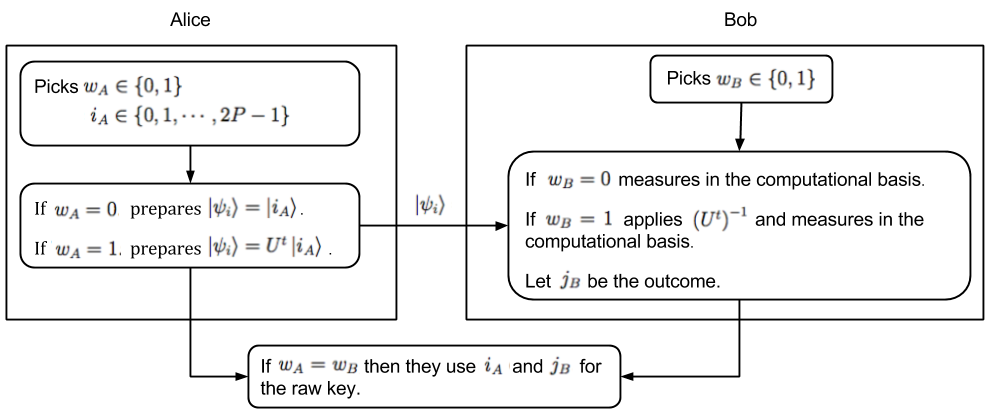
\includegraphics[width=\textwidth]{protocol_one-way.png}
\caption{Description of the basic steps of Protocol~\ref{alg:prot1}.}
\label{fig:prot1}
\end{figure}
\end{center}



\begin{protocol}
\label{alg:prot1}
Let $\theta_k, t,$ and $P$ be publicly known where $P$ is the dimension of the position space of the QW, $t$ is the number of steps to perform the QW, and $\theta_k$ the coin parameter (see Section~\ref{sec:secpk} for the exact form of $\theta_k$).  Let $U_k$ be the QW operator $U_k = S\cdot (I_p\otimes R_c(\theta_k))$ that is also known by the parties (i.e., it is also publicly known) and let $F$ be an operator acting only on $\mathcal{H}_c$. $F$'s action is to ``flip'' the coin to some initial state before evolving the walk and is optional (in which case $F=I_c$). Finally, let $\ket{\psi_i} = U_k^t(I_p\otimes F)\ket{i}$ for $\ket{i} \in \mathcal{H}_p\otimes\mathcal{H}_c$.  We call the orthonormal basis $\{\ket{\psi_i}\}$ the QW basis and denote the computational basis by $Z$.


The protocol consists of $N$ iterations of the following steps:
\begin{enumerate}
  \item $A$ picks a random bit $w_A \in \{0,1\}$ and a value $i_A \in \{0,1, \cdots, 2P-1\}$.
    \begin{itemize}
    \item If $w_A = 0$: $A$ will prepare and send to $B$ the $2P$-dimensional state $\ket{\psi_i} = \ket{i_A}$.
    \item If $w_A = 1$: $A$ will prepare and send to $B$ the $2P$-dimensional state $\ket{\psi_i} = U_k^t(I_p\otimes F)\ket{i_A}$.
    \end{itemize}

  \item $B$ picks a random bit $w_B \in \{0,1\}$.
    \begin{itemize}
    \item If $w_B = 0$: $B$ measures the received $2P$ dimensional state in the computational $Z$ basis resulting in outcome $j_B$.
    \item If $w_B = 1$: $B$ measures in the QW basis (alternatively, he inverts the QW by applying $\left(U_k^t\right)^{-1}$ and measures the resulting state in the $Z$ basis).  The result is translated, in the obvious way, into an integer $j_B$.
    \end{itemize}
Note that he measures both the position and coin, as opposite to the previous protocol, where the measurement for the key was only on the positions space.
  \item $A$ and $B$ reveal, via the authenticated classical channel, their choice of $w_A$ and $w_B$.  If $w_A = w_B$, they will use their values $i_A$ and $j_B$ to contribute towards their raw key.  Otherwise, if $w_A \ne w_B$, they will discard this iteration.
\end{enumerate}

After the above process, $A$ and $B$ will use a cut-and-choose technique similar to Yao's ~\cite{yao:86}, to check eavesdropping by choosing a suitable subset of non-discarded iterations for parameter estimation in the usual manner (discarding those chosen iterations from the raw key). This allows them to estimate the disturbance $Q_Z$ and $Q_W$ in the $Z$ and QW bases respectively (i.e., in the absence of noise $Q_Z = Q_W = 0$).  If this disturbance is ``sufficiently low'' (to be discussed below) the users proceed with error correction and privacy amplification in the usual manner.

\end{protocol}
\subsection{Security of the protocol}

In order to prove the security of Protocol~\ref{alg:prot1}, we will construct, in the usual way, an equivalent EB protocol~\cite{ben:bra:mer:92,lo:cha:99}. Proving security of this EB protocol will show the security of the PM version. For this EB version, for each one of the $N$ iterations, we make changes to steps (1) and (2), replacing them as follows:\vspace{5mm}

\textbf{New Step (1)}: $A$ prepares the entangled state:
\[
\ket{\phi_0} = \frac{1}{\sqrt{2P}}\sum_{i=0}^{2P-1}\ket{i,i}_{AB}
\]
which lives in the $4P^2$ dimensional Hilbert space: $\left(\mathcal{H}_p\otimes\mathcal{H}_c\right)^{\otimes 2}$.  She sends the second half (the $B$ portion of $\ket{\phi_0}$) to $B$ while keeping the first half (the $A$ portion) in her private lab. \vspace{5mm}

\textbf{New Step (2)}: $A$ and $B$ choose independently two random bits $w_A$ and $w_B$.  If $w_A = 0$, $A$ will measure her half of the entangled state in the computational $Z$ basis; otherwise she will measure her half in the QW basis.  Similarly for $B$ and $w_B$.  Let their measurement results in values be $i_A$ on $A$'s side and $j_B$ on $B$'s side.

We now show the security of this entanglement-based version of the protocol.  In the following proof, we will initially make three assumptions:
\begin{enumerate}
  \item[\bf A1:] $A$ and $B$ only use those iterations where $w_A = w_B = 0$ for their raw key.

  \item[\bf A2:] $E$ is restricted to collective attacks (those whereby she attacks each iteration of the protocol independently and identically, but is free to perform a joint measurement of her ancilla at any future time of her choosing).

  \item[\bf A3:] $E$ is the party that actually prepares the states which $A$ and $B$ hold.
\end{enumerate}

Assumption A1 is made only to simplify the computation and may be discarded later (alternatively, one may bias the basis choice so that $w_A$ and $w_B$ are chosen to be $0$ with high probability, thus increasing the efficiency of the protocol as is done for instance for BB84 in~\cite{lo:cha:ard:05}).  Assumption A2 may be removed later using a de Finetti-type argument~\cite{ren:gis:kra:05,chr:kon:ren:09,ren:07} (in this paper, we are only concerned with the asymptotic scenario, so the key-rate expression we derive will not be degraded). Note that removing A2 gives us the security. Assumption A3 gives greater advantage to the adversary; if we prove security using A3, then the ``real-world'' case, where assumption A3 is not used, will certainly be just as secure, if not even more.

In light of A2 and A3, $A$, $B$, and $E$, after $N$ iterations of the protocol, hold a quantum state $\rho_{ABE}^{\otimes N}$, where $\rho_{ABE} \in \mathcal{H}_A\otimes\mathcal{H}_B\otimes\mathcal{H}_E$ with $\mathcal{H}_A \equiv \mathcal{H}_B \equiv \mathcal{H}_p\otimes\mathcal{H}_c$.  Following error correction and privacy amplification, $A$ and $B$ will hold a secret key of size $\ell(N)$.  Under the assumption of collective attacks (A2), we may use the Devetak-Winter key-rate expression~\cite{dev:win:05} to compute:
\[
r = \lim_{N\rightarrow \infty}\frac{\ell(N)}{N} = S(A|E) - H(A|B).
\]

Let $A_Z$ and $A_W$ be the random variables describing $A$'s system, when she measures in the $Z$ or $QW$ basis, respectively.  Similarly, define $B_Z$ and $B_W$.  Under assumption A1, we are actually interested in the value:
\[
r = S(A_Z|E) - H(A_Z|B_Z).
\]

Computing $H(A_Z|B_Z)$ is trivial, given the observable probabilities:
%
\begin{equation}\label{eq:prot1:probZ}
p^Z_{i,j} = Pr(i_A=i \text{ and } j_B=j \text{ } | \text{ } w_A=w_B=0).
\end{equation}
%
The challenge is to determine a bound on the von Neumann entropy $S(A_Z|E)$.

To do so, we will use an uncertainty relation, proven in~\cite{ber:chr:col:ren:ren:10}, which states that for any density operator $\sigma_{ABE}$ acting on Hilbert space $\mathcal{H}_A\otimes\mathcal{H}_B\otimes\mathcal{H}_E$, if $A$ and $B$ make measurements using POVMs $\mathcal{M}_0 = \left\{M_x^{(0)}\right\}_x$ or $\mathcal{M}_1 = \left\{M_x^{(1)}\right\}_x$, then

\begin{equation}
S(A_0|E) + H(A_1|B) \ge \log\frac{1}{c},
\end{equation}

where

\begin{equation}
c = \max_{x,y}\left|\left| M_x^{(0)}M_y^{(1)} \right|\right|_\infty^2
\end{equation}
where we take $||\cdot||_\infty$ to be the operator norm and $A_i$ to be the random variable describing $A$'s system after measuring $\mathcal{M}_i$ (we will later, similarly, define $B_i$). Assuming measurements $\mathcal{M}_0$ are used for key distillation, simple algebra, as discussed in~\cite{ber:chr:col:ren:ren:10}, yields the Devetak-Winter key-rate:
\begin{eqnarray*}
r = S(A_0|E) - H(A_0|B_0)& \ge &\log\frac{1}{c} - H(A_0|B_0) - H(A_1|B)\\[2mm]
&\ge & \log\frac{1}{c} - H(A_0|B_0) - H(A_1|B_1).
\end{eqnarray*}
The last inequality follows from the basic fact that measurements can only increase entropy.

In our case, we have $M_x^{(0)} = \ket{x}\bra{x}$ and $M_x^{(1)} = \ket{\psi_x}\bra{\psi_x}$ for $x \in \left\{0, 1, \cdots, 2P-1\right\}$.  Let $\ket{\psi_x} = \sum_{i=0}^{2P-1}\alpha_{x,i}\ket{i}$; then it is easy to see that for all $x,y$
\[
\left|\left|M_x^{(0)}M_y^{(1)}\right|\right|_\infty^2 = |\alpha_{y,x}|^2,
\]
and therefore
\begin{equation}\label{eq:prot1:cval}
c = \max_{x,y}|\alpha_{x,y}|^2,
\end{equation}
a quantity which depends exclusively on the choice of the QW parameters and not on the noise in the channel. 
Therefore, $A$ and $B$ should choose optimal $t, \theta_k$ and $P$ in order to minimise $c$ (thereby maximising the key-rate equation).
As we will show in the next section, this analysis is sufficient to derive good key-rate bounds.

\subsection{Evaluation}
As mentioned above, the value of $c$ depends solely on the QW parameters which are under $A$ and $B$'s control; therefore it is to their advantage to choose a QW which minimises this value (i.e., such that, after evolving for $t$ steps, the probability of finding the walker at any particular position is small). 

 It is easy to see that, as $t \rightarrow \infty$, the values $|\alpha_{x,y}|$ do not converge to a steady state which is why, usually, one considers the time-averaged distribution when analysing QWs on the cycle~\cite{aha:amb:kem:vaz:01,kem:03}. 

However, in our QKD protocol, we do not care what happens at large $t$; instead, we wish to find an optimal $t$ and one that is preferably not ``too large'' (the larger it is, the longer, in general, it might take $A$ to prepare the state and $B$ to reverse it).

We begin by looking at various walk parameters and finding the minimal value of $c$ when $F=I_c$, the identity operator. Note that, on the circle, it makes sense only to consider odd $P$ as even $P$ would force the support of the probability amplitudes onto even or odd numbered nodes only thereby increasing the overall value of $|\alpha_{x,y}|$. We wrote a computer program to simulate the walk for time steps $t = 1, 2,\cdots , T_{\text{max}}$ (for user-specified value $T_{\text{max}}$) searching for the optimal value of $t$ (i.e., a value for $t$ whereby $c$ is minimum). For the evaluation we used a more general form of the coin rotation operator:

\begin{equation*}
R_c(\theta,\phi) = 	\left( 
				\begin{array}{cc}
					e^{i\phi} \cos(\theta) & e^{i\phi} \sin(\theta) \\
					-e^{-i\phi} \sin(\theta)& e^{-i\phi} \cos(\theta)
				\end{array}
			\right),
\end{equation*}

The results for $\theta = \pi/4, \phi = 0$, and for various $P$ are shown in Figure~\ref{fig:prot1:cvals}.
	
\begin{figure}[h!]
  \centering
  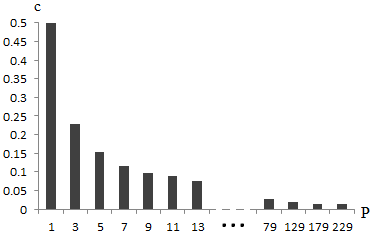
\includegraphics[scale = 0.6]{overlap-piover4.png}
\caption{Showing minimal value of $c$ found by our program for given position space dimension $P$ when $\theta = \pi / 4,\phi=0$ and $F=I_c$.  When $P \le 13$ we set $T_{\max} = 5000$; when $P \ge 79$ we set $T_{\max} = 50000$.  Note that, the smaller $c$ is, the better for $A$ and $B$.  Note also that $P$ is the dimension of the position space, \emph{not} the number of qubits sent which would actually be $\lceil\log P\rceil+1$ (where the extra ``$+1$'' is due to the coin).}\label{fig:prot1:cvals}
\end{figure}


Now that we can find the optimal choice of QW parameters for particular values of $P$ and, more importantly for our work here, the resulting value of $c$. To this end, we have to compute our bound $r$ and determine for what noise levels we can have $r > 0$.  
In practice, one would observe values $p_{i,j}^Z$ and $p_{i,j}^W$ (see Equation~\eqref{eq:prot1:probZ} and define $p_{i,j}^W$ analogously) and use these to directly compute $H(A_Z|B_Z)$ and $H(A_W|B_W)$ as required by the key-rate equation.  For the purpose of illustration in this paper, however, we will evaluate our key-rate bound assuming a generalised Pauli channel as discussed in~\cite{bae:aci:07} (see, in particular, Section~7 of that source). This channel maps an input state $\rho$ to an output state $\mathcal{E}(\rho)$ defined as:
\begin{equation}\label{eq:prot1-channel}
\mathcal{E}(\rho) = \sum_{m=0}^{2P-1}\sum_{n=0}^{2P-1}p_{m,n}\;\mathcal{U}_{m,n}\;\rho\;\mathcal{U}_{m,n}^*,
\end{equation}
where:
\begin{equation}
\mathcal{U}_{m,n} = \sum_{k=0}^{2P-1}e^{{\pi \cdot i \cdot  k \cdot n}/{P}}\ket{k+m}\bra{k},
\end{equation}
That is, this channel $\mathcal{E}(\cdot)$ models an adversary's attack which induces phase and flip errors with probabilities denoted by $p_{m,n}$.  In our numerical computations to follow, we will use:
\begin{equation}\label{eq:prot1-channelpr}
p_{i,j} = \left\{
\begin{array}{ll}
	1-E_r & \text{ if } i = j = 0\\[4mm]
	\ds \frac{E_r}{(2P)^2-1} & \text{ otherwise}
\end{array}
\right. .
\end{equation}
It is clear that $\sum_{i,j}p_{i,j} = 1$.  Furthermore, when $E_r=0$, we have $\sum_ip_{i,i}^Z = \sum_ip_{i,i}^W = 1$ (i.e., there is no disturbance in the channel) while as $E_r$ increases, the disturbance also increases.

Finally, we define the total noise in the channel to be:
\[
Q = \sum_{a\ne b}p_{a,b}^Z = \sum_{a\ne b} Pr \big( A_Z=a \text{ and } B_Z = b \text{ } | \text{ } w_A = w_B = 0 \big).
\]
That is to say, $Q$ represents the quantum error rate (QER) of the channel.

The maximally tolerated QER, for those QWs analysed in Figure~\ref{fig:prot1:cvals}, and using the above described noise model, is shown in Figure~\ref{fig:prot1:maxnoise1}.  Note that, when $P=1$ and $t=1$, we recover the BB84 limit of $11\%$ which is to be expected since, with these choice of parameters, we are essentially running the BB84 protocol.
\begin{figure}[h!]
  \centering
  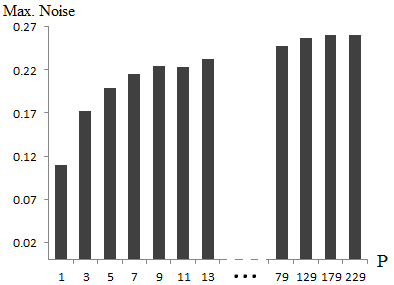
\includegraphics[scale=0.6]{maxNoisePiOver4.png}
\caption{Showing the maximally tolerated noise level for our protocol using parameters found in Figure~\ref{fig:prot1:cvals} and using the quantum channel described by Equations~\eqref{eq:prot1-channel} and~ \eqref{eq:prot1-channelpr}. The lack of increase in noise tolerance from $P=9$ to $P=11$ (while other choices caused an increase) indicates that $T_{\max}$ was too low.  Note that, when $P = 1$, we recover the BB84 tolerance of $Q = 0.11$ as expected.  Also note that, when $P = 229$, the maximal tolerated noise is $Q = 0.261$.}\label{fig:prot1:maxnoise1}
\end{figure}
Observe in Figure~\ref{fig:prot1:maxnoise1} that there is a lack of increase when $P=9$ and $P=11$; this indicates that our choice of $T_{\max} = 5000$ was too low.  Running our simulator again with $T_{\max} = 50000$ for these small $P$ values yields a maximally tolerated noise level shown in Figure~\ref{fig:prot1:maxnoise2}.

\begin{figure}[h!]
  \centering
  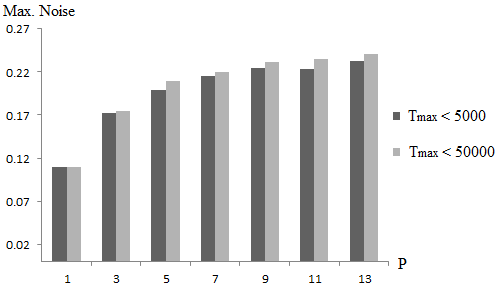
\includegraphics[scale=0.60]{maxNoiseBigT.png}
\caption{Comparing the maximally tolerated noise when $t$ is allowed to be as large as $50000$ (light gray) or only $5000$ (dark grey); again when $F = I$ and $\phi = 0$.  In this case, when $P=13$ and $T_{\max} = 50000$, the maximal tolerated noise $Q$ is $Q = 0.241$.}\label{fig:prot1:maxnoise2}
\end{figure}

Finally, we re-run the simulator, using $T_{\max} = 5000$ and $T_{\max} = 50000$ for a different QW parameter of $\theta = \sqrt{2}\pi/4$ which, for these particular upper-bounds on $t$ yield a higher tolerated noise as shown in Figures~\ref{fig:prot1:walk2} and\ref{fig:prot1:walk2-2}.  
We comment that, if $T_{\max}$ were larger, the two QWs may produce a QKD protocol with the same tolerated noise; however for these ``smaller'' bounds on $t$ the QW with parameter $\theta = \sqrt{2}\pi/4$ produces a more secure protocol than when $\theta = \pi/4$.  Since smaller $t$ implies a more efficient protocol, this is an advantage.  This opens two very interesting questions: first, do these QWs produce equivalent noise tolerances as $T_{\max}\rightarrow \infty$? Second, what other values of $\theta$ produce even more secure QKD protocols for small $T_{\max}$?  We comment that we also ran this numerical experiment for $\theta = \pi/5$ and $\theta = \pi/3$ but got worse noise tolerances.

\begin{figure}[h!]
  \centering
  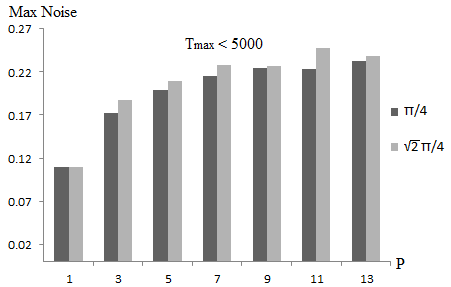
\includegraphics[scale = 0.60]{maxNoiseCompare.png}
\caption{Comparing the maximal tolerated noise levels of the QKD protocol when $\theta = \pi/4$ (dark gray) and $\theta = \sqrt{2}\pi/4$ (light grey).  In this chart, $T_{\max} = 5000$ which, observing the ``drop'' in tolerated noise when $P$ goes from 11 to 13, is too small.  See also Figure~\ref{fig:prot1:walk2-2} for the same chart when $T_{\max} = 50000$.}\label{fig:prot1:walk2}
\end{figure}

\begin{figure}[h!]
  \centering
  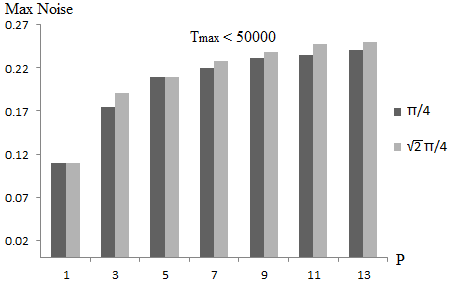
\includegraphics[scale = 0.60]{maxNoiseCompareBigT.png}
\caption{Comparing the maximal tolerated noise levels of the QKD protocol when $\theta = \pi/4$ (dark gray) and $\theta = \sqrt{2}\pi/4$ (light grey).  In this chart, $T_{\max} = 50000$.  In all cases, the QW parameter $\theta = \sqrt{2}\pi/4$ produces a more secure QKD protocol for this upper-bound on $t$.  Note that, as $T_{\max} \rightarrow \infty$, they may produce equally secure protocols; this, as discussed in the text, is an open question.  In this case, when $P=13$ and $\theta = \sqrt{2}\pi/4$, the maximally tolerated noise is $0.25$ (compared to $0.241$ when $\theta = \pi/4$).}\label{fig:prot1:walk2-2}
\end{figure}


From the above it is clear that careful choice of the QW parameters is vital for producing a QKD protocol tolerant of high noise channels.  To investigate this further, we simulate the QW for all $\theta,\phi \in \{k\pi/10 \text{ } | \text{ } k = 0, 1, \cdots, 10\}$.  Furthermore, for each setting, we also consider the use of $F = I, F = X$, and $F = Y$, where:
\[
\begin{array}{clc}
X = \ds \frac{1}{\sqrt{2}}\left(
			\begin{array}{cc}
					1 & 1\\
					1 & -1
			\end{array}\right)
& &
Y = \ds \frac{1}{\sqrt{2}}\left(
			\begin{array}{cc}
					1 & 1\\
					i & -i
			\end{array}\right).
\end{array}
\]	


For each setting, we find the optimal choice of time $t \le 5000$ which produces a minimal $c$.  We then take this value and determine the highest disturbance the resulting protocol can withstand.  The respective data is summarised in Table~\ref{table:sim-results}.

\begin{center}
	\begin{table*}[h!]
		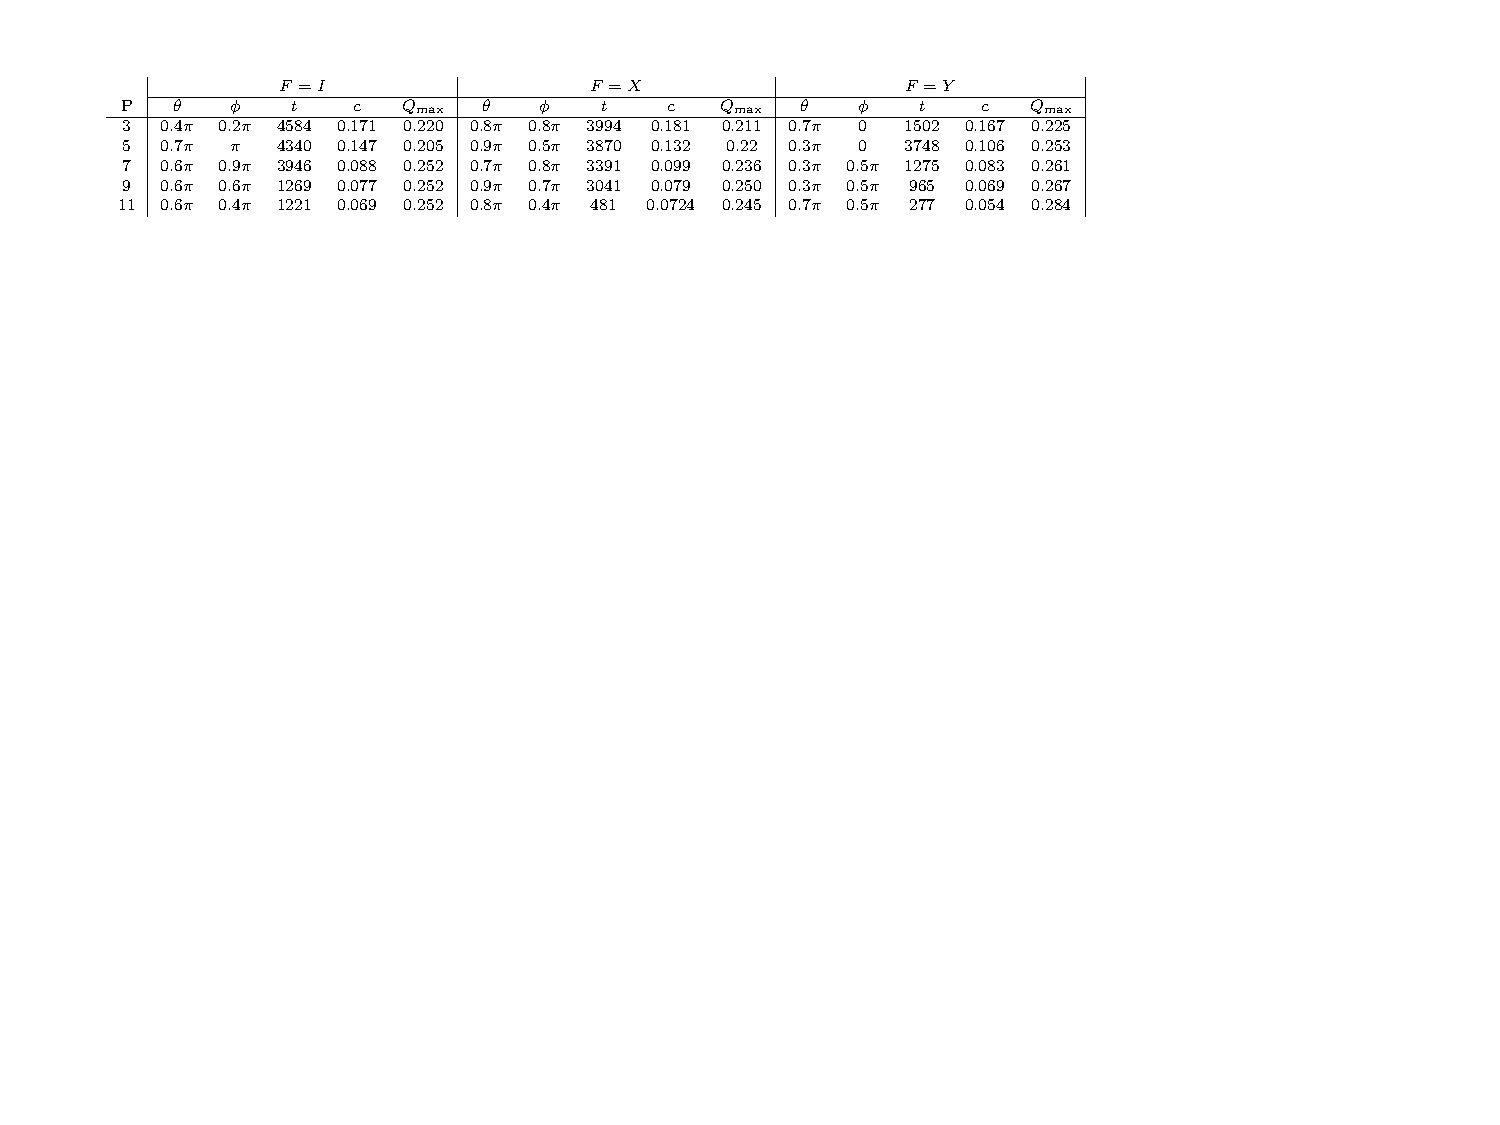
\includegraphics[scale = 1.1]{Table1}
		\caption{Showing the optimal choice of QW parameters to maximise the noise tolerance ($Q_{\text{max}}$) of the resulting protocol.  For this data, we searched for QWs with at most $T_{\text{max}} = 5000$ steps and with parameters $\theta,\phi \in \{k\pi/10 \text{ } | \text{ } k = 0, 1, \cdots, 10\}$.}\label{table:sim-results}
	\end{table*}
\end{center}

Note that, for some data points (e.g., when $P = 5$ and $F = I$) there is a drop in the maximum tolerated noise.  This is a consequence either of setting $T_{\text{max}}$ too small, or we need to simulate more QW parameters. For example, when we set $T_{\max} = 50000$, for $P = 5$ and $F = I$, we get a maximum noise tolerance of $0.236$ when $t = 40847$.  Note also, that setting $F = Y$ achieves the best result for this test, $Q_{\text{max}}=0.284$.\\

In Table~\ref{table:sim-results2}, we carried out the same experiment, however this time searching over QW parameters in the set $\theta, \phi \in \{k\pi/20 \text{ } | \text{ } k = 0, 1, \cdots, 20\}$. Again, the best result for this case is $Q_{\text{max}}=0.284$ and is achieved when considering $F = Y$. 

\begin{center}
	\begin{table*}[h!]
		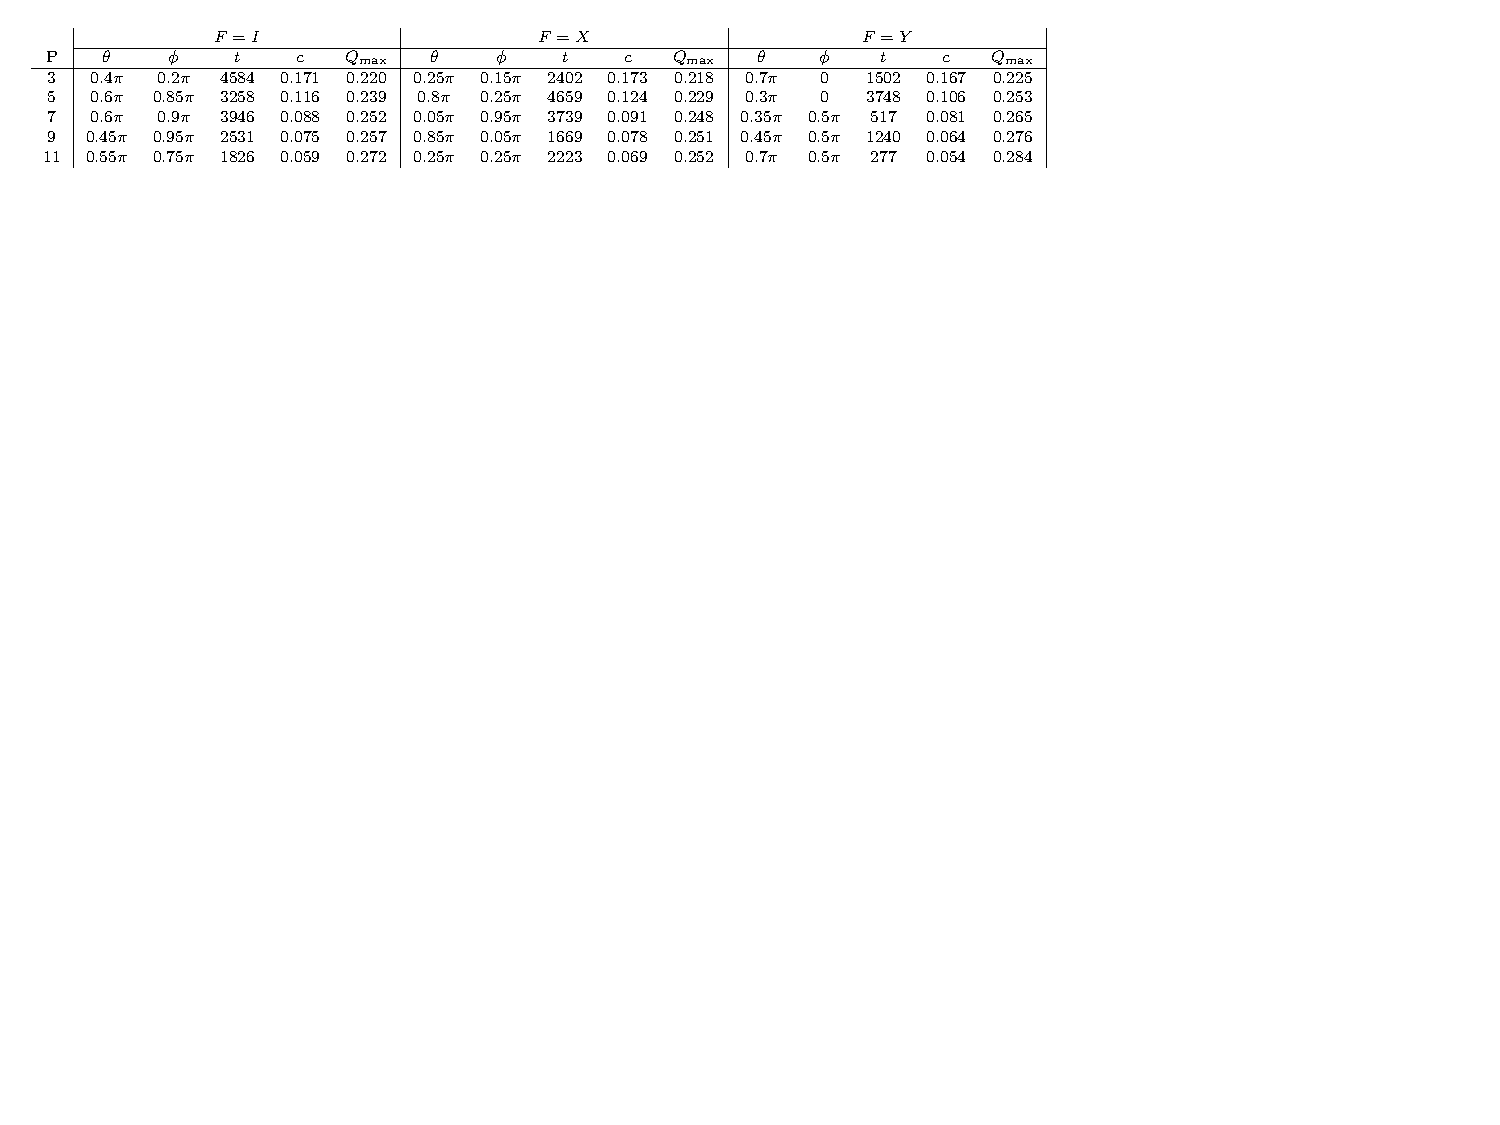
\includegraphics{Table2.pdf}
		\caption{Showing the optimal choice of QW parameters to maximise the noise tolerance ($Q_{\text{max}}$) of the resulting protocol.  For this data, we searched for QWs with at most $T_{\text{max}} = 5000$ steps and with parameters $\theta,\phi \in \{k\pi/20 \text{ } | \text{ } k = 0, 1, \cdots, 20\}$.}\label{table:sim-results2}
	\end{table*}
\end{center}

As mentioned at the beginning of this section, all the numerical results were obtained by simulating the evolution of the QW on a custom QW simulator that we wrote. However, we also verified the results through an alternative technique, namely by computing the probability amplitudes of the QW using the standard Fourier method (see, e.g.~\cite{nay:vis:00,ven:and:12}) of analysing QWs. The results obtained by both methods agree with each other.\\

Finally, we note that the protocol's security is not compromised by considering the existence or not of quantum memories. It is sufficient to consider the PM form of the protocol. $E$ needs a quantum memory to perform her attack, as she needs to save her ancillary system throughout the execution of the protocol. In the contrary, the secure key distribution between $A$ and $B$ does not require any quantum memory. Therefore, if $E$ does not have a quantum memory she cannot attack, while if even she has one and attacks, $A$ and $B$ can defend against it and securely share a key at the end. Notice, that even if we consider the EB version of the protocol, again the security is independent of any quantum memory requirements, as $E$ for her attack needs a more stable quantum memory than $A$ and $B$ need to defend against it and securely distil the key.  

\newpage

\section{Semi-quantum key distribution protocol}
\label{sec:semi-qkdscheme}

As a third contribution, in this section, we propose a new \emph{semi-quantum} key-distribution (SQKD) protocol based on QWs.  The concept of semi-quantum cryptography was introduced by Boyer {\em et al.}~\cite{boy:ken:mor:07,boy:gel:ken:mor:09}, as a way to study ``how quantum'' does a protocol need to be in order to surpass the security of its classical counterparts -- namely, how ``quantum'' do the parties need to be in order to establish a secret key secure against an all-powerful adversary.  A semi-quantum protocol places restrictions on one of the participating users (typically $B$) in that he may only operate in a ``classical'' or ``semi-quantum'' manner. In particular, this limited user -- usually called the {\em classical party} -- can only directly work with the computational basis.  No restrictions are placed on $A$, who is fully quantum, i.e., she possesses quantum equipment and can perform quantum operations and of course, no restrictions are placed on $E$. Implementation-wise, such protocols can be seen as practical instances of QKD, since they involve less quantum hardware. 
 Semi-quantum protocols rely on a two-way quantum channel allowing a quantum state to travel from $A$ to $B$, and then back to $A$.  When first introduced by Boyer {\em et al.} in \cite{boy:ken:mor:07}, these classical operations involved $B$ either measuring the incoming qubit in the $Z = \{\ket{0}, \ket{1}\}$ basis, or reflecting the incoming qubit, bouncing it back to $A$ undisturbed.  For our purposes, we extend this definition of ``classical'' operations to operate with higher dimensional systems.  As we do not want to restrict ourselves necessarily to qubit encodings (and thus, dimensions that are powers of two), we will say that $B$, on receipt of an $D$ dimensional quantum state $\ket{\psi},$ may choose to do one of two operations:
\begin{enumerate}
  \item Measure and Resend: $B$ may subject the $D$-dimensional quantum state to a measurement in the computational basis spanned by states: $\{\ket{0}, \ket{1}, \cdots,$ $ \ket{D-1}\}$.  He will then prepare a new $D$-dimensional quantum state in this same computational basis based on the result of his measurement.  Namely, if he observes $\ket{r}$ for $r \in \{0, 1, \cdots, D-1\}$, he will send to $A$ the quantum state $\ket{r}$.
  \item Reflect: $B$ may ignore the incoming $D$-dimensional quantum state and reflect it back to $A$.  In this case he learns nothing about its state.
\end{enumerate}

With these restrictions on the part of the classical user defined, we now depict our protocol in Figure~\ref{fig:semi_QKD} and describe it immediately below.


    \begin{center}
    \begin{figure}[h!]
    \centering
    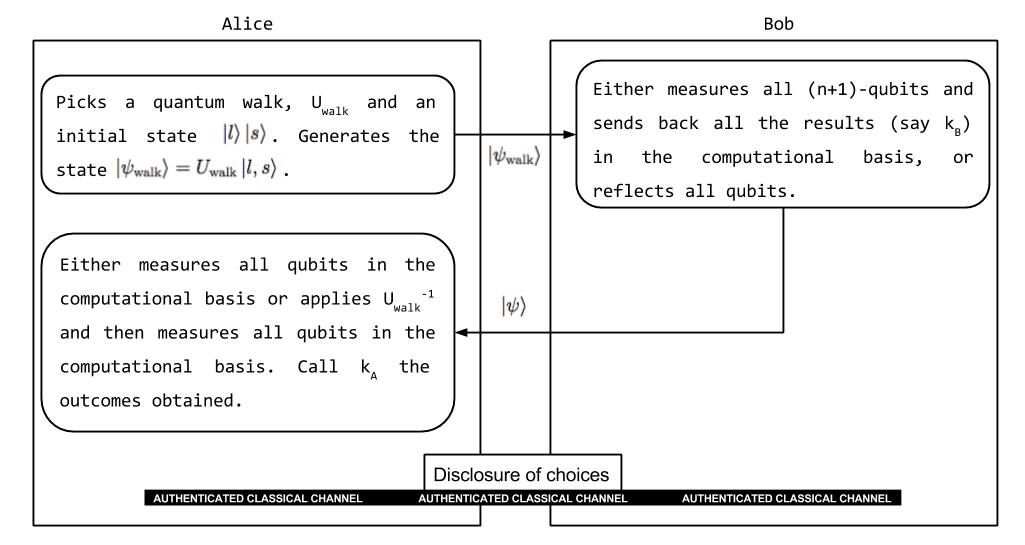
\includegraphics[width=0.8\textwidth]{semi_quantum_QKD.png}
    \caption{Description of the basic steps of Protocol~\ref{prot:semi-q}.}
    \label{fig:semi_QKD}
    \end{figure}
    \end{center}

\newpage
\begin{protocol} Semi-quantum key-distribution scheme\
\label{prot:semi-q} 
\begin{description}
\item[\hspace{6mm}{\bf Inputs for the protocol} ]\
\begin{itemize}
	\item $\ket{l,s}$, the initial state of the QW, where $l \in \mathcal L=\{ 0, \dots, P-1 \} $ is the initial position of the walker, and $s \in \mathcal S=\{R,L\}$ gives the initial coin state.
	\item $U_{\textnormal{walk}} = (U_k)^t \in \mathcal Q$, the evolution of the QW, where $k \in \mathcal K  =\{1,2,\ldots,K\}$ is the choice of a single step unitary $U_k$, and $t \in \mathcal{T} = \{ T_0, \dots, T_{max} \}$ is the number of steps of the QW. Thus, $\mathcal Q$ is the set of all possible QWs. Note that $\mathcal Q$  is publicly known.
\end{itemize}

\vspace{3mm}
\item[\hspace{6mm}{\bf Quantum state Generation}]\
\begin{itemize}
 \item $A$ chooses uniformly at random $l \in \mathcal L=\{0,1,\cdots, P-1\}$ and $s\in\mathcal S=\{R,L\}$.  She also chooses a random QW operator $U_{\textnormal{walk}} \in \mathcal{Q}$ according to a publicly known distribution (e.g., uniform).  She then prepares the following state:

$$\ket{\psi_{\textnormal{walk}}} = U_{\textnormal{walk}}\ket{l,s}.$$
\item $A$ sends this state to $B$.
\end{itemize}

\vspace{3mm}
 \item[\hspace{6mm}{ \bf Classical operations by $B$} ]\
 
 
  $B$ chooses either to measure-and-resend the quantum state in the computational basis $\{\ket{0}, \ket{1}, \cdots, \ket{2P-1}\}$ (note that, in this protocol as well, he measures both the position and coin in order to obtain the key, thus his measurement, and subsequent preparation, is of dimension $2P$); or he will reflect the quantum state back to $A$.

\vspace{3mm}

  \item[\hspace{6mm}{\bf $A$'s final step} ]\
  
  $A$ chooses one of the following two options:
  \begin{itemize}
  	\item She measures the returning quantum state in the computational basis and saves the result as $\kappa_A$. 
  	\item She first applies the inverse QW, $U_{\textnormal{walk}}^{-1}$, and then measures in the computational basis. Note that, in the absence of noise, if $B$ reflects, her measurement outcome should be $\ket{l,s}$.
   \end{itemize}

\vspace{3mm}
  \item[\hspace{6mm}{\bf Disclosure}]\
   
  $A$ discloses her choice of operation and $B$ discloses his choice either to measure and resend or reflect.
  
  \vspace{3mm}
   \item[\hspace{6mm}{\bf Iterations} ]\
   
  The above process is repeated $N$ times. 
  
  \vspace{3mm}
   \item[\hspace{6mm}{\bf Results} ]\
  \begin{itemize}
  	\item Every time $B$ measures and resends and $A$ measures in the computational basis, the parties add $1+\log P$ bits  to their final raw key.  
  	\item Every time $B$ reflects and $A$ measures after applying the inverse QW, the outcome of her measurement $(l_m,s_m)$ should be what she initially used to generate the QW state (i.e., it should be that $l=l_m$ and $s=s_m$). These iterations, together with some randomly chosen iterations of the first type (where $B$ measures and resends), are used for error detection. 
  	\item The other iterations are discarded.
  \end{itemize}
\end{description}
\end{protocol}

\subsection{Proof of robustness}

As with the first protocol we proposed in this section, the reliance on a two-way quantum channel greatly complicates the security analysis.  It was only recently that several SQKD protocols were proven secure~\cite{krawec2015security,krawec2016security,krawec2016quantum,zha:qiu:mat:16}. However, the proof techniques developed in those works assumed qubit-level systems.  In our case, not only must we contend with the two-way channel, but also with the fact that the quantum states traveling between $A$ and $B$ are of dimensions higher than $2$.  This leads to significant challenges in the security analysis. Therefore, as a first step, we will prove that the protocol is \emph{robust}, as defined in~\cite{boy:ken:mor:07,boy:gel:ken:mor:09}. That is, for any attack which $E$ may perform which causes her to gain information on the raw key, this attack must necessarily lead to a disturbance in the channel which can be detected with non-zero probability by $A$ and $B$. 

\begin{theorem}\label{thm:sqkd-robust}
If $I \in \mathcal{Q}$ (where $I$ is the identity operator on the joint $2P$ dimensional system) and if, for every $(l,s), (l',s') \in \{0,1,\cdots, P-1\}\times\{R,L\}$ there exists a $U_{\textnormal{walk}} \in \mathcal{Q}$ and initial state $\ket{l_0,s_0}$ (all possibly depending on the choice of $(l,s)$ and $(l',s')$) such that $\braket{l,s|U_{\textnormal{walk}}|{l_0,s_0}} \ne 0$ and $\braket{l',s'|U_{\textnormal{walk}}|l_0,s_0} \ne 0$, then the SQKD protocol based on QWs is robust.
\end{theorem}
\begin{proof}

We will assume, similarly to~\cite{zou:qiu:li:wu:li:09,kra:14}, that $A$ sends each (in our case $2P$-dimensional) quantum state, only after she receives one from $B$ (excepting, of course, the first iteration).  In this case, $E$'s most general attack consists of a collection of unitary operators $\left\{(U_F^{(i)}, U_R^{(i)})\right\}_{i=1}^N$ where, on iteration $i$ of the protocol, she applies $U_F^{(i)}$ in the forward channel (as the quantum state travels from $A$ to $B$) and $U_R^{(i)}$ in the reverse channel.  These operators act on the $2P$-dimensional quantum state and $E$'s private quantum memory.  We make no assumptions about how these operators are chosen -- for instance, $E$ may choose them ``on the fly''; that is, she may choose operator $U_F^{(2)}$ after attacking with $U_F^{(1)}$.

Consider the first iteration $i=1$.  We assume, without loss of generality, that $E$'s quantum memory is cleared to some pure ``zero'' state, denoted by $\ket{\chi}$, known to her.

In the remainder of this proof, we will treat the position space and the coin space as a single space $\Sigma$ of dimension $2P$.

We may describe the action of $U_F^{(1)}$ on basis states as follows
\[
U_F^{(1)}\ket{i, \chi} = \sum_{j=0}^{2P-1}\ket{j, e_i^j},
\]
where $\ket{e_i^j}$ are arbitrary states in $E$'s ancillary system. These states are not necessarily normalised nor orthogonal; the unitarity of $U_F^{(1)}$ imposes some restrictions on them which we will use later.

With non-zero probability, this iteration may be used for error detection.  It is also possible that $A$ chose to use $I \in \mathcal{Q}$ in this iteration and, thus, she sends the quantum state $\ket{\sigma}$ to $B$, for $\sigma \in \Sigma$. Furthermore, $B$ chooses to measure and resend with non-zero probability. Therefore, to avoid detection, it must be that $\ket{e_i^j}\equiv 0$ for all $i \ne j$, and the unitarity of  $U_F^{(1)}$ yields $\braket{e_i^i|e_i^i} = 1$ for all $i$.  Thus:
\[
U_F^{(1)} \ket{i,\chi} = \ket{i,e_i^i}, \forall i=0,1,\cdots,2P-1.
\]
Now, consider $U_R^{(1)}$, the attack applied in the reverse channel.  We may write its action as follows:
\[
U_R^{(1)}\ket{i, e_i^i} = \sum_{w=0}^{2P-1}\ket{w, e_{i,i}^w}.
\]
The same argument as before applies: in particular, with non-zero probability $A$ and $B$ will use this iteration to check for errors, and so it must be that $\ket{e_{i,i}^w} \equiv 0 $ for $i \ne w$.  Thus
\[
U_R^{(1)}\ket{i, e_i^i} = \ket{i, e_{i,i}^i} = \ket{i, f_i}, \forall i = 0,1,\cdots, 2P-1,
\]
where we defined $\ket{f_i} \equiv \ket{e_{i,i}^i}$ for ease of notation.

Now, assume that $A$ chooses a QW operator $\walkop \in \mathcal{Q}$, with $\walkop \ne I$.  Let $\ket{\sigma}$ be the initial state she prepares ($\sigma$ chosen at random from $\Sigma$).  In this case, the quantum state she sends to $B$ may be written as:
\[
\walkop\ket{\sigma} = \ket{\psi_\sigma} = \sum_{i=0}^{2P-1}\alpha_i\ket{i}.
\]
Assume that $\walkop$ is chosen so that at least two of the $\alpha_i$'s are non-zero (such QWs exist by hypothesis).  If $B$ reflects, the qubit state arriving at $A$'s lab, after $E$'s attack on both channels, is
\begin{equation}\label{eq:wk:walkresult}
U_R^{(1)}U_F^{(1)}(\walkop\otimes I_E)\ket{\sigma,\chi} = \sum_i \alpha_i\ket{i,f_i},
\end{equation}
where $I_E$ is the identity operator on $E$'s ancilla.

$A$ will subsequently apply the inverse QW operator and measure the resulting state, expecting to find $\ket{\sigma}$.  This is equivalent to her measuring in the QW basis $\{\ket{\psi_0}, \ket{\psi_1}, \cdots, \ket{\psi_{2P-1}}\}$, where $\ket{\psi_i} = \walkop\ket{i}$, and expecting to observe $\ket{\psi_\sigma}$.  In this QW basis, we clearly have
\[
\ket{i} = \sum_{j=0}^{2P-1}\braket{\psi_j|i}\ket{\psi_j},
\]
from which, we may write Equation~\eqref{eq:wk:walkresult} as:
\begin{eqnarray}
\sum_{i=0}^{2P-1}\alpha_i \left( \sum_{j=0}^{2P-1}\braket{\psi_j|i}\ket{\psi_j}\right) \otimes \ket{f_i}\\\\
=\sum_{j=0}^{2P-1}\ket{\psi_j}\otimes\left(\sum_{i=0}^{2P-1}\alpha_i\braket{\psi_j|i}\ket{f_i}\right).
\end{eqnarray}
Let $p$ be the probability that this iteration does not result in an error -- i.e., the probability that $A$ measures $\ket{\psi_\sigma}$. From the above equation:
\[
p = \left| \sum_{i=0}^{2P-1}\alpha_i\braket{\psi_\sigma|i}\ket{f_i} \right|^2.
\]
Noticing that $\braket{\psi_\sigma|i} = \alpha_i^*$ (since $\ket{\psi_\sigma} = \sum_i\alpha_i\ket{i}$), and also $\braket{f_i|f_i} = 1$ (due to the unitarity of $U_R^{(1)}$), we find:
\[
p = \left|\sum_i|\alpha_i|^2\ket{f_i}\right|^2 = \sum_i|\alpha_i|^4 + 2\sum_{i>j\ge 0}|\alpha_i|^2|\alpha_j|^2\text{Re}(\braket{f_i|f_j}).
\]

When $\ket{f_i} \equiv \ket{f_j}=\ket{F},$ for all $i,j$, the above quantity attains its maximum of $p=1$. In this case, after $E$'s attack, the system described by Equation~\eqref{eq:wk:walkresult} is $\sum_i\alpha_i\ket{i}\otimes\ket{F} = \ket{\psi_\sigma}\otimes\ket{F}$.  Due to the Cauchy-Schwarz inequality $\text{Re}(\braket{f_i|f_j}) \le 1$.  If, however, one or more of the $\text{Re}(\braket{f_i|f_j}) < 1$ for any of the $(\ket{f_i}, \ket{f_j})$ pairs which appear in the expression above (i.e., for those where $\alpha_i$ and $\alpha_j$ are non-zero), it is obvious that $p < 1$ and so $E$ would be detected.

Therefore, to avoid detection, it must be that $\text{Re}(\braket{f_i|f_j}) = 1$ for all $i,j$ where $\alpha_i$ and $\alpha_j$ are non-zero, implying $\ket{f_i} \equiv \ket{f_j}$.  Indeed, if we write $\ket{f_j} = x\ket{f_i} + y\ket{\zeta}$, where $\braket{f_i|\zeta} = 0$, then $\text{Re}(\braket{f_i|f_j}) = 1 = \text{Re} (x)$.  Of course $|x|^2 + |y|^2 = 1$ (since $\braket{f_j|f_j} = 1$) and so:
\begin{equation*}
|x|^2+|y|^2 = 1\\
\Rightarrow \text{Re}^2 x + \text{Im}^2 x + |y|^2 = 1\\
\Rightarrow \text{Im}^2x + |y|^2 = 0.
\end{equation*}
This implies both $\text{Im}(x) = 0$ and $y=0$.  Since $\text{Re}(x) = 1$, we conclude $x=1$ and so $\ket{f_i} = \ket{f_j}$.

Since $A$ could have chosen any QW in $\mathcal{Q}$, all possible $(i,j)$ pairs are covered (i.e., at least one QW in $\mathcal{Q}$ is guaranteed to produce a state where $\alpha_i$ and $\alpha_j$ are non-zero) and since $E$ does not know which QW was chosen, it must be that $\ket{f_i} \equiv \ket{f_j} \equiv \ket{F}$ for all $i,j$.

Thus, after the first iteration, to avoid detection, it must be that the state of $E$'s quantum memory is in the state $\ket{F}$, independently of $A$'s and $B$'s raw key and operations.  Thus, $E$ is not able to extract any information during the first iteration. Furthermore, since she is fully aware of the state of her quantum memory in this case (i.e., she knows the state $\ket{F}$), the above arguments may be repeated inductively for the remaining iterations of the protocol, leading to the conclusion that the protocol is robust.
\end{proof}

The above proof of robustness placed certain requirements on the set of QW $\mathcal{Q}$, but can such a set even exist?  We show that, at least for all odd $P$, such a set may be easily constructed.

\begin{lemma}
If $P$ is odd, then there exists a set of QWs $\mathcal{Q}$ which satisfy the requirements of Theorem \ref{thm:sqkd-robust}.
\end{lemma}
\begin{proof}
Let $(l,s),(l',s') \in \{0,1,\cdots, P-1\}\times\{R,L\}$.  We construct a QW $U_{l,s,l',s'}$ and an initial state $\ket{l_0,s_0}$ such that $\braket{l,s|U_{l,s,l',s'}|l_0,s_0} \ne 0$ and $\braket{l',s'|U_{l,s,l',s'}|l_0,s_0} \ne 0$.

Since $P$ is odd, there exits a position index $q \in \{0,1,\cdots,P-1\}$ and a value $q_0 \in \mathbb{Z}$ such that $|q_0| < P$, $q-q_0 \equiv l \text{ (mod) } P$, and $q+q_0\equiv l' \text{ (mod) } P$.  We assume that $q_0 \ge 0$; if $q_0 < 0$ the result is symmetric by simply ``flipping'' $l$ with $l'$ (in which case $q_0$ becomes non-negative).

The shift operator $S$ for our QW is simply the usual
\[
S = \sum_{i=0}^{P-1}\ket{i-1}\bra{i}\otimes \ket{R}\bra{R} + \sum_{i=0}^{P-1}\ket{i+1}\bra{i} \otimes \ket{L}\bra{L},
\]
where all arithmetic, of course, is done modulo $P$.  Our coin operator will simply be the Hadamard coin:
\[
R_c = \frac{1}{\sqrt{2}}\left(
\begin{array}{cc}
1&1\\
1&-1
\end{array}\right).
\]
We claim the desired operator is $U_{l,s,l',s'} = \left[ ( I_p\otimes R_c)\cdot S\right]^{t+1}$. (Note that the shift operator is applied before the coin in this case to simplify the construction) Now, consider the initial state $\ket{q+1,R}$.  After the first step of the QW (i.e., after applying $(I_p\otimes R_c)\cdot S$), the QW evolves to the state $\frac{1}{\sqrt{2}}\ket{q}(\ket{R}+\ket{L})$.  It is not difficult to see that, after $t$ additional steps with this QW, \emph{but before the final application of $I_p\otimes R_c$ on the $(t+1)$-th step}, the quantum state evolves to:
\[
\alpha\ket{l,R} + \beta\ket{l',L} + \ket{\phi},
\]
where $|\alpha| \ne 0, |\beta| \ne 0$, and $\ket{\phi}$ is a non-normalised state orthogonal to both $\ket{l,R}$ and $\ket{l',L}$.  Finally, after the last $I_p\otimes R_c$, the state becomes
\begin{eqnarray*}
U_{l,s,l',s'}\ket{q+1,R} = \frac{1}{\sqrt{2}}(\alpha\ket{l,R} + \alpha\ket{l,L} \\+ \beta\ket{l',R} - \beta\ket{l',L}) + \ket{\phi'},
\end{eqnarray*}
with $\ket{\phi'}$ being a state orthogonal to $\ket{l,R}, \ket{l,L}, \ket{l',R},$ and $\ket{l',L}$, thus yielding the desired state.  Taking $\mathcal{Q} = \bigcup_{l,s,l',s'}\left\{U_{l,s,l',s'}\right\} \cup \{I\}$ proves the result.
\end{proof}

Finally, we should notice that the robustness of this SQKD protocol is independent of the existence or absence of  quantum memories. In fact, $E$'s attack requires a stable quantum memory, in which she keeps her ancillary system during the execution of the protocol. On the other hand, $A$ does not need any quantum memory in order to share the key with $B$ at the end, and $B$ is, of course, restricted to classical operations. Therefore, without a quantum memory $E$ cannot even conduct the attack, whereas even if she has access to a quantum memory, she is not able to extract any useful information about the key without being detected by $A$ and $B$.


\section{Practical attacks}
\label{sec:prac_att}

While our work includes theoretical cryptographic proposals, and a detailed analysis of practical attacks is out of its scope, it is worthy presenting a short discussion of possible attacks and countermeasures for the case of optical implementations. The term practical attacks refers to attacks during which $E$ is taking advantage of possible loopholes in the implementation of the protocols, i.e., the fact that the setups used for the implementation of the protocols are not perfect, can seriously compromise the security of the key. Such attacks have been thoroughly investigated in the literature and several countermeasures have been proposed in different setups and scenarios. For an overview of the recent progress and current status of this area of QKD, see the following detailed reviews~\cite{sca:bsc:csr:dus:lut:pee:09,jai:sti:kha:els:mar:leu:16,dia:lo:qi:yua:16,bed:arr:lin:17,dix:etal:17}.

One of the most studied of such attacks is the photon number splitting attack (PNS), which is based on the fact that there are no perfect single-photon sources~\cite{bra:lut:mor:san:00,lut:00,lut:jah:02}. Instead, the current sources emit in general multi-photon pulses, whose photon number statistics are described by a Poisson distribution. $E$, who is considered all-powerful and bounded only by the laws of physics, can thus, by placing herself in front of $A$, detect genuine multi-photon pulses, extract one photon from each, and send the rest to $B$ through a lossless channel, while blocking single-photon pulses. Due to the fact that the quantum channel connecting $A$ and $B$ has losses exponential in the channel length, there exists a maximal distance, known to $E$, below which $E$ is not able to spot $E$'s interference. By storing the extracted photons in her quantum memory, $E$ can measure them in the correct basis upon the classical communication between $A$ and $B$, during which they publicly reveal their choices of preparation/measurement bases. Since all the photons of the same pulse are in the same state, $E$ thus has the key shared by $A$ and $B$.

The standard technique used to defend against a PNS attack is by introducing the so-called decoy states~\cite{hwa:03}. In addition to the signal states, from which the key is obtained, $A$ sends coherent states $\ket{e^{i\theta}|\alpha|}$, with phase $\theta$ chosen uniformly at random, and the variable intensity $I\propto |\alpha|$. Note that such decoy pulses are to $E$ indistinguishable from the signal ones. Thus, $A$ and $B$ can subsequently detect $E$'s interference (extracting single photons from multi-photon pulses) by comparing the yields of signal and decoy states (given the channel loss $\ell$, the yield $y$ is defined as $y=1-\ell$~\cite{hwa:03}). For more details, see~\cite{lo:ma:che:05}, as well as subsequent improvements and modifications~\cite{wan:05a,wan:05b,har:ett:hug:nor:05,ma:qi:zha:lo:05,wan:wan:bjo:kar:07,ros:pet:har:ric:dal:tya:mcc:nam:bae:had:hug:nor:09,luc:dyn:fro:yua:shi:15}. This method, developed for standard one-way QKD schemes, can be straightforwardly applied to our second proposal, which is a one-way protocol as well. It can also be applied to our first and third two-way proposals. Indeed, in our first proposal, as $B$ does not perform any measurement, it is $A$ who performs the yield estimation upon receiving back the pulses. The same can be done by $A$ alone for the photons reflected by $B$ in our third proposal, in which in addition the yield check could be done for the pulses measured by $B$. As mentioned above, the details of the techniques depend on particular implementations and are beyond the scope of our theoretical study.

While the PNS attack is applicable to most of the protocols that use imperfect photon sources, the above description of its particular implementation is given on the example of a standard QKD {\em one-way} scheme. Thus, it has to be re-examined when applied to different protocols. The crucial feature of the standard QKD protocol is the exchange of classical information between $A$ and $B$, which allows $E$ to extract the key exchanged. Therefore, since such exchange is present in our second and third protocol, the above described PNS attack is applicable to those protocols as well. Note though that in the case of the third, {\em two-way} protocol, $E$ can possibly extract information only upon intercepting the pulses re-sent from $B$ to $A$. Indeed, in the third protocol the key is obtained from the cases in which $B$ and, upon receiving them back, $A$ too, perform measurements in the computational basis, thus sharing the same set of bits. Extracting photons from the pulse before it came to $B$, and consequently before his measurement, gives $E$ no information about the key.

Nevertheless, our first, {\em two-way} QKD protocol, is considerably different from the standard QKD ones, as $A$ and $B$ reveal {\em no classical information} regarding their quantum operations (they only exchange information regarding the cases used for verification procedure, which do not contribute to the key generation). Thus, $E$'s task is more difficult than in the case of standard QKD protocols. What $E$ can do is to extract {\em two} photons from each pulse, one on the way from $A$ to $B$, and another on the way back to $A$, and compare their states, $\ket\psi$ and $\ket{\psi(r)}$, in the attempt to learn the key $r$. Note that, even in the noiseless scenario, the described comparison does not have perfect efficiency, unlike the standard application of the PNS attack in which $E$ learns the key with certainty. Moreover, in the case of our protocol, $E$ can attack only three or more photon pulses, thus decreasing the efficiency of her attack with respect to the standard one, which makes use of more probable two-photon pulses as well. For example, for the commonly used order of the mean photons per pulse, $\mu = 0.2$, the probability for emitting three or more photons is $p(n\geq 3) \approx 0.001$, while the probability to emit exactly two photons (the ``deficit'' with respect to the standard PNS attack) is of the order of magnitude higher, $p(n=2) \approx 0.016$, where $n$ is the number of photons per pulse emitted. 

Finally, we would like to note that, although in practical attacks $E$ is assumed to be all powerful, exceeding the current technological equipment used by everyday users, not all practical attacks are based on the same level of subtle equipment. In the case of the PNS attack, $E$ should be able to perform photon non-demolition number measurements, a task beyond any current and (at least mid-term) foreseeable technology.

Nevertheless, there exist other practical protocols that do not requite such sophisticated technology. Below, we briefly analyse three such kinds of attacks, extensively studied in the literature: the Trojan horse, the detector blinding and the time-shift attacks.

The Trojan horse attack is one of the first attacks ever considered and since then it has been thoroughly investigated and continuously developed in different contexts. In a nutshell, Trojan horse attacks benefits from the imperfections in the quantum channel between $A$ and $B$ that allows for $E$'s interference by modulating $A$'s pulses, sending them to $B$ and analysing the reflected/backscattered signal~\cite{vak:mak:hje:01,luc:cho:war:dyn:yua:shi:15,saj:min:jai:mak:17}. The first such attack benefitted from the detector imperfections, by collecting the light emitted upon the detection of the photons~\cite{kur:zar:may:wei:01}. To counter such attacks, introducing simple optical isolators suffice in one-way protocols, while for two-way protocols one needs to introduce additional monitoring detectors~\cite{gis:fas:kra:zbi:rib:06}.

Furthermore, we would like to briefly discuss two more attacks, namely the detector blinding and the time-shift attacks, which are both considered in the broader context of intercept and resend with faked states attacks~\cite{liz:lop:lop:16}.  In general, during an intercept and resend with faked states attack, $E$ is not trying to extract information about the key from the original states that the legitimate parties exchange. Instead, she generates and sends to them classical or quantum light pulses, which are tailored in a way that she can control their measurement outcomes, while she is blocking the original states. At the end of such an attack, $E$ and the legitimate parties share the same key, without $A$ and $B$ being able to detect her interference. In both the aforementioned attacks, $E$ is taking advantage of loopholes in the performance and efficiency of the detectors of the legitimate parties. 

First, we consider the detector blinding attacks to standard one-way QKD protocols~\cite{lyd:wie:wit:els:ska:mak:10,wie:lyd:wit:els:ska:mar:mak:leu:11}. $E$ first intercepts the state that $A$ sends to $B$ and measures it in one of the two possible bases, that she randomly chooses. Then, she sends to one of $B$'s detectors a bright light pulse according to her measurement outcome. Note that the intensity of the bright light pulse is just a bit above the detector's threshold. If $B$ chooses to measure in the same basis as $E$, all the light will be directed to one of his detectors, due to the interference. The detector, which is now operating in the linear instead of the Geiger mode (avalanche photon diode), will click and $E$ will now share the same key bit with $B$. If $B$ chooses to measure in the complementary basis, the light will be divided in two components and its intensity will not be enough to trigger neither of the the detectors, therefore $B$ will not get a click and this iteration will be discarded. Subsequently, $A$ and $B$ will keep for the key the bits for which $A$'s preparation basis and $B$'s measuring basis agree. During their classical communication, $E$ will learn exactly which are these bits, therefore she will share the same key, while her interference remains unnoticed. 

This attack is ineffective for the case of our first, two-way, protocol, in which only $A$ is performing the measurement on the pulses received back from $B$. Note that her performing the inverse QW, followed by the measurement in the computational basis, is equivalent to measuring in an {\em unknown} to $E$ (ensured by our Holevo argument mentioned in Section~\ref{sec:sec2way}, and presented with details in Chapter 2), ``rotated'' basis, with respect to the computational one. Therefore, virtually all $E$'s attempts to perform the detector blinding attack would result in no detection events for $A$. Moreover, even the (rare) detections, being uncorrelated with the initial state sent by $A$, would not pass the verification procedure described in Section~\ref{sec:stdver}, as well as the analogous checking rounds of the third, two-way semi-quantum protocol (when $B$ reflects the pulses back to $A$ and she performs the inverse walk and measures in the computational basis).

Regarding our second, one-way key distribution protocol, $B$'s action is similar to the one in the standard protocols: he measures in one of the two publicly known bases. To counter such an attack, $B$ can apply one of the known counter-measures proposed and analysed in~\cite{liu:lin:kur:ska:mak:ger:14,sti:14,ele:ozh:kur:gol:mak:15,wan:wan:qin:wei:zha:16,lee:par:woo:par:kim:han:moo:16}. Nevertheless, we would like to note again that our QW protocol is more complex than the standard ones based on few (typically four) quantum states, and thus its implementations might possibly invoke new challenges, a topic worth a separate study. 

Time-shift attacks take advantage of the different timing responses of the detectors. Assuming $E$ knows the timings of during which each detector is (in)sensitive, allows her to, similarly as in the previous case of the detector blinding, enforce the particular outcomes of $B$'s/$A$'s measurements. Analogously as in the case of detector blinding attacks, such strategy cannot pass the two-way verification procedures and checking rounds of our first and  third protocols. In the case of our one-way protocol, one could employ similar methods to the ones proposed in~\cite{mak:ani:ska:06,lam:kur:07,zha:fun:qi:che:lo:08,qi:fun:lo:ma:07}, in order to defend against a time-shift attack. 

\newpage
\section{Conclusions}
In the work presented in this chapter, we employed, for the first time to the best of our knowledge, QWs in order to design and analyze new secure QKD protocols. Besides the theoretically interesting intersection of two unique and fascinating fields of quantum information science, there are also potential practical benefits in pursuing this investigation. Some high-dimensional QKD protocols have the ability to withstand a high noise tolerance, as recently shown in several studies~\cite{bec:tit:00,cer:bou:kar:gis:02,bru:chr:eke:eng:ber:kas:mac:03,nik:alb:05,she:sca:10,cha:15}. Here we proposed QKD protocols based on high-dimensional states generated by means of QWs, and we showed that they are more tolerant to noise compared to protocols based on two-dimensional states. Apart from their interesting theoretical properties, it could be that, in a future quantum infrastructure, the generation of these QW states would be easier compared to other higher-dimensional systems. Indeed, producing such states may not need the high entanglement of many qubits -- instead they could be generated through the evolution of a single-qubit walker on, for instance, a multi-node quantum network.

In what follows, we point out some directions of future work. First, it would be interesting to perform a more detailed study on the two verification procedures presented in Section~\ref{sec:sec2way} and compare them with respect to various attack strategies. Moreover, one could analyse the relation between the two for concrete cases of $E$'s cheating strategies in the presence of noise.\\
In Section~\ref{sec:oneway}, we proved the security of the one-way protocol, but still some improvements could be done. In particular, one could find an analytical solution for the optimal choice of QW parameters or, alternatively, given particular QW parameters, to find an analytical solution for the value of $c$ from Equation~\eqref{eq:prot1:cval}. Another interesting question would be to understand the maximally tolerated noise as the dimension of the position space and the number of steps of the QW go to infinity. For instance, in~\cite{cha:15} a high-dimensional QKD protocol was introduced (not using QWs, but simpler states), which could suffer a bit error rate of up to $50\%$ as the dimension of the state sent by $A$ approached infinity. Can we construct a QW-QKD protocol with similar features?  Does our protocol approach this disturbance level for high $P$?

Moreover, studying and employing other QW models (perhaps the memory-based QWs described and analysed in, e.g.,~\cite{get:10,get:jar:mis:14,roh:bre:gil:13,kra:15,aha:amb:kem:vaz:01,bru:car:amb:03}) or QWs on different graphs, would be interesting -- our key-rate equation would generalize to these cases; the only change would be the value of $c$. Perhaps different QW models, or different graphs, would produce more optimal values, thus increasing the key rate.

Finally, the SQKD protocol we proposed lacks of a proof of security beyond robustness. As we already mentioned in Section~\ref{sec:semi-qkdscheme}, this proof is technically very challenging due to the high-dimensional QW states and the use of a two-way channel. Hence, computing analytically the key rate is extremely hard.  Moreover, the numerical simulation is equally challenging, even for low-dimensional walks. Nevertheless, we believe that obtaining the key rate is not impossible, and we expect that this analysis will yield quite high error-tolerance. A first step towards this direction would be to try to reduce this protocol to a simpler one (for instance, the one in~\cite{boy:ken:mor:07}, for which there is a security proof~\cite{krawec2015security}) and prove that it is at least as secure. This reduction does not seem to be a straightforward task and requires a thorough analysis.


%
%\bibliography{bibforthesis}
%\bibliographystyle{unsrt}
%
%\end{document}
